\documentclass[12pt,a4paper]{report}
\usepackage{graphicx,iman,extra,ttbox,pdfsetup}

\title{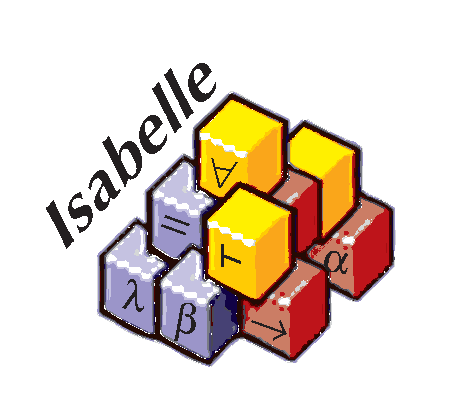
\includegraphics[scale=0.5]{isabelle} \\[4ex] Old Isabelle Reference Manual}

\author{{\em Lawrence C. Paulson}\\
        Computer Laboratory \\ University of Cambridge \\
        \texttt{lcp@cl.cam.ac.uk}\\[3ex] 
        With Contributions by Tobias Nipkow and Markus Wenzel}  

\setcounter{secnumdepth}{2} \setcounter{tocdepth}{2}

\pagestyle{headings}
\sloppy
\binperiod     %%%treat . like a binary operator

\begin{document}
\underscoreoff

\index{definitions|see{rewriting, meta-level}}
\index{rewriting!object-level|see{simplification}}
\index{meta-rules|see{meta-rules}}

\maketitle 
\emph{Note}: this document is part of the earlier Isabelle
documentation and is mostly outdated.  Fully obsolete parts of the
original text have already been removed.  The remaining material
covers some aspects that did not make it into the newer manuals yet
\cite{isabelle-isar-ref,isabelle-implementation}.

\subsubsection*{Acknowledgements} 
Tobias Nipkow, of T. U. Munich, wrote most of
  Chapters~\protect\ref{Defining-Logics} and~\protect\ref{chap:simplification}.
  Markus Wenzel contributed to Chapter~\protect\ref{chap:syntax}.
  Jeremy Dawson, Sara Kalvala, Martin
  Simons  and others suggested changes
  and corrections.  The research has been funded by the EPSRC (grants
  GR/G53279, GR/H40570, GR/K57381, GR/K77051, GR/M75440) and by ESPRIT
  (projects 3245: Logical Frameworks, and 6453: Types), and by the DFG
  Schwerpunktprogramm \emph{Deduktion}.

\pagenumbering{roman} \tableofcontents \clearfirst


\chapter{Syntax primitives}

The rather generic framework of Isabelle/Isar syntax emerges from three main
syntactic categories: \emph{commands} of the top-level Isar engine (covering
theory and proof elements), \emph{methods} for general goal refinements
(analogous to traditional ``tactics''), and \emph{attributes} for operations
on facts (within a certain context).  Here we give a reference of basic
syntactic entities underlying Isabelle/Isar syntax in a bottom-up manner.
Concrete theory and proof language elements will be introduced later on.

\medskip

In order to get started with writing well-formed Isabelle/Isar documents, the
most important aspect to be noted is the difference of \emph{inner} versus
\emph{outer} syntax.  Inner syntax is that of Isabelle types and terms of the
logic, while outer syntax is that of Isabelle/Isar theory sources (including
proofs).  As a general rule, inner syntax entities may occur only as
\emph{atomic entities} within outer syntax.  For example, the string
\texttt{"x + y"} and identifier \texttt{z} are legal term specifications
within a theory, while \texttt{x + y} is not.

\begin{warn}
  Old-style Isabelle theories used to fake parts of the inner syntax of types,
  with rather complicated rules when quotes may be omitted.  Despite the minor
  drawback of requiring quotes more often, the syntax of Isabelle/Isar is
  somewhat simpler and more robust in that respect.
\end{warn}

Printed theory documents usually omit quotes to gain readability (this is a
matter of {\LaTeX} macro setup, say via \verb,\isabellestyle,, see also
\cite{isabelle-sys}).  Experienced users of Isabelle/Isar may easily
reconstruct the lost technical information, while mere readers need not care
about quotes at all.

\medskip

Isabelle/Isar input may contain any number of input termination characters
``\texttt{;}'' (semicolon) to separate commands explicitly.  This is
particularly useful in interactive shell sessions to make clear where the
current command is intended to end.  Otherwise, the interpreter loop will
continue to issue a secondary prompt ``\verb,#,'' until an end-of-command is
clearly recognized from the input syntax, e.g.\ encounter of the next command
keyword.

Advanced interfaces such as Proof~General \cite{proofgeneral} do not require
explicit semicolons, the amount of input text is determined automatically by
inspecting the present content of the Emacs text buffer.  In the printed
presentation of Isabelle/Isar documents semicolons are omitted altogether for
readability.

\begin{warn}
  Proof~General requires certain syntax classification tables in order to
  achieve properly synchronized interaction with the Isabelle/Isar process.
  These tables need to be consistent with the Isabelle version and particular
  logic image to be used in a running session (common object-logics may well
  change the outer syntax).  The standard setup should work correctly with any
  of the ``official'' logic images derived from Isabelle/HOL (including HOLCF
  etc.).  Users of alternative logics may need to tell Proof~General
  explicitly, e.g.\ by giving an option \verb,-k ZF, (in conjunction with
  \verb,-l ZF, to specify the default logic image).
\end{warn}

\section{Lexical matters}\label{sec:lex-syntax}

The Isabelle/Isar outer syntax provides token classes as presented below; most
of these coincide with the inner lexical syntax as presented in
\cite{isabelle-ref}.

\indexoutertoken{ident}\indexoutertoken{longident}\indexoutertoken{symident}
\indexoutertoken{nat}\indexoutertoken{var}\indexoutertoken{typefree}
\indexoutertoken{typevar}\indexoutertoken{string}\indexoutertoken{altstring}
\indexoutertoken{verbatim}
\begin{matharray}{rcl}
  ident & = & letter\,quasiletter^* \\
  longident & = & ident (\verb,.,ident)^+ \\
  symident & = & sym^+ ~|~ \verb,\<,ident\verb,>, \\
  nat & = & digit^+ \\
  var & = & ident ~|~ \verb,?,ident ~|~ \verb,?,ident\verb,.,nat \\
  typefree & = & \verb,',ident \\
  typevar & = & typefree ~|~ \verb,?,typefree ~|~ \verb,?,typefree\verb,.,nat \\
  string & = & \verb,", ~\dots~ \verb,", \\
  altstring & = & \backquote ~\dots~ \backquote \\
  verbatim & = & \verb,{*, ~\dots~ \verb,*}, \\[1ex]

  letter & = & latin ~|~ \verb,\<,latin\verb,>, ~|~ \verb,\<,latin\,latin\verb,>, ~|~ greek ~|~ \\
         &   & \verb,\<^isub>, ~|~ \verb,\<^isup>, \\
  quasiletter & = & letter ~|~ digit ~|~ \verb,_, ~|~ \verb,', \\
  latin & = & \verb,a, ~|~ \dots ~|~ \verb,z, ~|~ \verb,A, ~|~ \dots ~|~ \verb,Z, \\
  digit & = & \verb,0, ~|~ \dots ~|~ \verb,9, \\
  sym & = & \verb,!, ~|~ \verb,#, ~|~ \verb,$, ~|~ \verb,%, ~|~ \verb,&, ~|~  %$
   \verb,*, ~|~ \verb,+, ~|~ \verb,-, ~|~ \verb,/, ~|~ \\
  & & \verb,<, ~|~ \verb,=, ~|~ \verb,>, ~|~ \verb,?, ~|~ \texttt{\at} ~|~
  \verb,^, ~|~ \verb,_, ~|~ \verb,|, ~|~ \verb,~, \\
greek & = & \verb,\<alpha>, ~|~ \verb,\<beta>, ~|~ \verb,\<gamma>, ~|~ \verb,\<delta>, ~| \\
      &   & \verb,\<epsilon>, ~|~ \verb,\<zeta>, ~|~ \verb,\<eta>, ~|~ \verb,\<theta>, ~| \\
      &   & \verb,\<iota>, ~|~ \verb,\<kappa>, ~|~ \verb,\<mu>, ~|~ \verb,\<nu>, ~| \\
      &   & \verb,\<xi>, ~|~ \verb,\<pi>, ~|~ \verb,\<rho>, ~|~ \verb,\<sigma>, ~| \\
      &   & \verb,\<tau>, ~|~ \verb,\<upsilon>, ~|~ \verb,\<phi>, ~|~ \verb,\<psi>, ~| \\
      &   & \verb,\<omega>, ~|~ \verb,\<Gamma>, ~|~ \verb,\<Delta>, ~|~ \verb,\<Theta>, ~| \\
      &   & \verb,\<Lambda>, ~|~ \verb,\<Xi>, ~|~ \verb,\<Pi>, ~|~ \verb,\<Sigma>, ~| \\
      &   & \verb,\<Upsilon>, ~|~ \verb,\<Phi>, ~|~ \verb,\<Psi>, ~|~ \verb,\<Omega>, \\
\end{matharray}

The syntax of $string$ admits any characters, including newlines; ``\verb|"|''
(double-quote) and ``\verb|\|'' (backslash) need to be escaped by a backslash.
Alternative strings according to $altstring$ are analogous, using single
back-quotes instead.  The body of $verbatim$ may consist of any text not
containing ``\verb|*}|''; this allows convenient inclusion of quotes without
further escapes.  The greek letters do \emph{not} include \verb,\<lambda>,,
which is already used differently in the meta-logic.

Common mathematical symbols such as $\forall$ are represented in Isabelle as
\verb,\<forall>,.  There are infinitely many legal symbols like this, although
proper presentation is left to front-end tools such as {\LaTeX} or
Proof~General with the X-Symbol package.  A list of standard Isabelle symbols
that work well with these tools is given in \cite[appendix~A]{isabelle-sys}.

Comments take the form \texttt{(*~\dots~*)} and may be nested, although
user-interface tools may prevent this.  Note that \texttt{(*~\dots~*)}
indicate source comments only, which are stripped after lexical analysis of
the input.  The Isar document syntax also provides formal comments that are
considered as part of the text (see \S\ref{sec:comments}).

\begin{warn}
  Proof~General does not handle nested comments properly; it is also unable to
  keep \verb,(*,\,/\,\verb,{*, and \verb,*),\,/\,\verb,*}, apart, despite
  their rather different meaning.  These are inherent problems of Emacs
  legacy.  Users should not be overly aggressive about nesting or alternating
  these delimiters.
\end{warn}


\section{Common syntax entities}

Subsequently, we introduce several basic syntactic entities, such as names,
terms, and theorem specifications, which have been factored out of the actual
Isar language elements to be described later.

Note that some of the basic syntactic entities introduced below (e.g.\
\railqtok{name}) act much like tokens rather than plain nonterminals (e.g.\
\railnonterm{sort}), especially for the sake of error messages.  E.g.\ syntax
elements like $\CONSTS$ referring to \railqtok{name} or \railqtok{type} would
really report a missing name or type rather than any of the constituent
primitive tokens such as \railtok{ident} or \railtok{string}.


\subsection{Names}

Entity \railqtok{name} usually refers to any name of types, constants,
theorems etc.\ that are to be \emph{declared} or \emph{defined} (so qualified
identifiers are excluded here).  Quoted strings provide an escape for
non-identifier names or those ruled out by outer syntax keywords (e.g.\
\verb|"let"|).  Already existing objects are usually referenced by
\railqtok{nameref}.

\indexoutertoken{name}\indexoutertoken{parname}\indexoutertoken{nameref}
\indexoutertoken{int}
\begin{rail}
  name: ident | symident | string | nat
  ;
  parname: '(' name ')'
  ;
  nameref: name | longident
  ;
  int: nat | '-' nat
  ;
\end{rail}


\subsection{Comments}\label{sec:comments}

Large chunks of plain \railqtok{text} are usually given \railtok{verbatim},
i.e.\ enclosed in \verb|{*|~\dots~\verb|*}|.  For convenience, any of the
smaller text units conforming to \railqtok{nameref} are admitted as well.  A
marginal \railnonterm{comment} is of the form \texttt{--} \railqtok{text}.
Any number of these may occur within Isabelle/Isar commands.

\indexoutertoken{text}\indexouternonterm{comment}
\begin{rail}
  text: verbatim | nameref
  ;
  comment: '--' text
  ;
\end{rail}


\subsection{Type classes, sorts and arities}

Classes are specified by plain names.  Sorts have a very simple inner syntax,
which is either a single class name $c$ or a list $\{c@1, \dots, c@n\}$
referring to the intersection of these classes.  The syntax of type arities is
given directly at the outer level.

\railalias{subseteq}{\isasymsubseteq}
\railterm{subseteq}

\indexouternonterm{sort}\indexouternonterm{arity}
\indexouternonterm{classdecl}
\begin{rail}
  classdecl: name (('<' | subseteq) (nameref + ','))?
  ;
  sort: nameref
  ;
  arity: ('(' (sort + ',') ')')? sort
  ;
\end{rail}


\subsection{Types and terms}\label{sec:types-terms}

The actual inner Isabelle syntax, that of types and terms of the logic, is far
too sophisticated in order to be modelled explicitly at the outer theory
level.  Basically, any such entity has to be quoted to turn it into a single
token (the parsing and type-checking is performed internally later).  For
convenience, a slightly more liberal convention is adopted: quotes may be
omitted for any type or term that is already atomic at the outer level.  For
example, one may just write \texttt{x} instead of \texttt{"x"}.  Note that
symbolic identifiers (e.g.\ \texttt{++} or $\forall$) are available as well,
provided these have not been superseded by commands or other keywords already
(e.g.\ \texttt{=} or \texttt{+}).

\indexoutertoken{type}\indexoutertoken{term}\indexoutertoken{prop}
\begin{rail}
  type: nameref | typefree | typevar
  ;
  term: nameref | var
  ;
  prop: term
  ;
\end{rail}

Positional instantiations are indicated by giving a sequence of terms, or the
placeholder ``$\_$'' (underscore), which means to skip a position.

\indexoutertoken{inst}\indexoutertoken{insts}
\begin{rail}
  inst: underscore | term
  ;
  insts: (inst *)
  ;
\end{rail}

Type declarations and definitions usually refer to \railnonterm{typespec} on
the left-hand side.  This models basic type constructor application at the
outer syntax level.  Note that only plain postfix notation is available here,
but no infixes.

\indexouternonterm{typespec}
\begin{rail}
  typespec: (() | typefree | '(' ( typefree + ',' ) ')') name
  ;
\end{rail}


\subsection{Mixfix annotations}

Mixfix annotations specify concrete \emph{inner} syntax of Isabelle types and
terms.  Some commands such as $\TYPES$ (see \S\ref{sec:types-pure}) admit
infixes only, while $\CONSTS$ (see \S\ref{sec:consts}) and
$\isarkeyword{syntax}$ (see \S\ref{sec:syn-trans}) support the full range of
general mixfixes and binders.

\indexouternonterm{infix}\indexouternonterm{mixfix}\indexouternonterm{structmixfix}
\begin{rail}
  infix: '(' ('infix' | 'infixl' | 'infixr') string? nat ')'
  ;
  mixfix: infix | '(' string prios? nat? ')' | '(' 'binder' string prios? nat ')'
  ;
  structmixfix: mixfix | '(' 'structure' ')'
  ;

  prios: '[' (nat + ',') ']'
  ;
\end{rail}

Here the \railtok{string} specifications refer to the actual mixfix template
(see also \cite{isabelle-ref}), which may include literal text, spacing,
blocks, and arguments (denoted by ``$_$''); the special symbol \verb,\<index>,
(printed as ``\i'') represents an index argument that specifies an implicit
structure reference (see also \S\ref{sec:locale}).  Infix and binder
declarations provide common abbreviations for particular mixfix declarations.
So in practice, mixfix templates mostly degenerate to literal text for
concrete syntax, such as ``\verb,++,'' for an infix symbol, or ``\verb,++,\i''
for an infix of an implicit structure.



\subsection{Proof methods}\label{sec:syn-meth}

Proof methods are either basic ones, or expressions composed of
methods via ``\texttt{,}'' (sequential composition), ``\texttt{|}''
(alternative choices), ``\texttt{?}'' (try), ``\texttt{+}'' (repeat at
least once), ``\texttt{[$n$]}'' (restriction to first $n$ sub-goals,
default $n = 1$).  In practice, proof methods are usually just a comma
separated list of \railqtok{nameref}~\railnonterm{args}
specifications.  Note that parentheses may be dropped for single
method specifications (with no arguments).

\indexouternonterm{method}
\begin{rail}
  method: (nameref | '(' methods ')') (() | '?' | '+' | '[' nat? ']')
  ;
  methods: (nameref args | method) + (',' | '|')
  ;
\end{rail}

Proper Isar proof methods do \emph{not} admit arbitrary goal
addressing, but refer either to the first sub-goal or all sub-goals
uniformly.  The goal restriction operator ``\texttt{[$n$]}'' evaluates
a method expression within a sandbox consisting of the first $n$
sub-goals (which need to exist).  For example,
$simp_all\mbox{\tt[}3\mbox{\tt]}$ simplifies the first three
sub-goals, while $(rule~foo, simp_all)\mbox{\tt[]}$ simplifies all new
goals that emerge from applying rule $foo$ to the originally first
one.

Improper methods, notably tactic emulations, offer a separate
low-level goal addressing scheme as explicit argument to the
individual tactic being involved.  Here $[!]$ refers to all goals, and
$[n-]$ to all goals starting from $n$,

\indexouternonterm{goalspec}
\begin{rail}
  goalspec: '[' (nat '-' nat | nat '-' | nat | '!' ) ']'
  ;
\end{rail}


\subsection{Attributes and theorems}\label{sec:syn-att}

Attributes (and proof methods, see \S\ref{sec:syn-meth}) have their own
``semi-inner'' syntax, in the sense that input conforming to
\railnonterm{args} below is parsed by the attribute a second time.  The
attribute argument specifications may be any sequence of atomic entities
(identifiers, strings etc.), or properly bracketed argument lists.  Below
\railqtok{atom} refers to any atomic entity, including any \railtok{keyword}
conforming to \railtok{symident}.

\indexoutertoken{atom}\indexouternonterm{args}\indexouternonterm{attributes}
\begin{rail}
  atom: nameref | typefree | typevar | var | nat | keyword
  ;
  arg: atom | '(' args ')' | '[' args ']'
  ;
  args: arg *
  ;
  attributes: '[' (nameref args * ',') ']'
  ;
\end{rail}

Theorem specifications come in several flavors: \railnonterm{axmdecl} and
\railnonterm{thmdecl} usually refer to axioms, assumptions or results of goal
statements, while \railnonterm{thmdef} collects lists of existing theorems.
Existing theorems are given by \railnonterm{thmref} and \railnonterm{thmrefs},
the former requires an actual singleton result.  There are three forms of
theorem references: (1) named facts $a$, (2) selections from named facts $a(i,
j - k)$, or (3) literal fact propositions using $altstring$ syntax
$\backquote\phi\backquote$, (see also method $fact$ in
\S\ref{sec:pure-meth-att}).

Any kind of theorem specification may include lists of attributes both on the
left and right hand sides; attributes are applied to any immediately preceding
fact.  If names are omitted, the theorems are not stored within the theorem
database of the theory or proof context, but any given attributes are applied
nonetheless.

\indexouternonterm{axmdecl}\indexouternonterm{thmdecl}
\indexouternonterm{thmdef}\indexouternonterm{thmref}
\indexouternonterm{thmrefs}\indexouternonterm{selection}
\begin{rail}
  axmdecl: name attributes? ':'
  ;
  thmdecl: thmbind ':'
  ;
  thmdef: thmbind '='
  ;
  thmref: (nameref selection? | altstring) attributes?
  ;
  thmrefs: thmref +
  ;

  thmbind: name attributes | name | attributes
  ;
  selection: '(' ((nat | nat '-' nat?) + ',') ')'
  ;
\end{rail}


\subsection{Term patterns and declarations}\label{sec:term-decls}

Wherever explicit propositions (or term fragments) occur in a proof text,
casual binding of schematic term variables may be given specified via patterns
of the form ``$\ISS{p@1\;\dots}{p@n}$''.  There are separate versions
available for \railqtok{term}s and \railqtok{prop}s.  The latter provides a
$\CONCLNAME$ part with patterns referring the (atomic) conclusion of a rule.

\indexouternonterm{termpat}\indexouternonterm{proppat}
\begin{rail}
  termpat: '(' ('is' term +) ')'
  ;
  proppat: '(' ('is' prop +) ')'
  ;
\end{rail}

Declarations of local variables $x :: \tau$ and logical propositions $a :
\phi$ represent different views on the same principle of introducing a local
scope.  In practice, one may usually omit the typing of $vars$ (due to
type-inference), and the naming of propositions (due to implicit references of
current facts).  In any case, Isar proof elements usually admit to introduce
multiple such items simultaneously.

\indexouternonterm{vars}\indexouternonterm{props}
\begin{rail}
  vars: (name+) ('::' type)?
  ;
  props: thmdecl? (prop proppat? +)
  ;
\end{rail}

The treatment of multiple declarations corresponds to the complementary focus
of $vars$ versus $props$: in ``$x@1~\dots~x@n :: \tau$'' the typing refers to
all variables, while in $a\colon \phi@1~\dots~\phi@n$ the naming refers to all
propositions collectively.  Isar language elements that refer to $vars$ or
$props$ typically admit separate typings or namings via another level of
iteration, with explicit $\AND$ separators; e.g.\ see $\FIXNAME$ and
$\ASSUMENAME$ in \S\ref{sec:proof-context}.


\subsection{Antiquotations}\label{sec:antiq}

\begin{matharray}{rcl}
  theory & : & \isarantiq \\
  thm & : & \isarantiq \\
  prop & : & \isarantiq \\
  term & : & \isarantiq \\
  const & : & \isarantiq \\
  abbrev & : & \isarantiq \\
  typeof & : & \isarantiq \\
  typ & : & \isarantiq \\
  thm_style & : & \isarantiq \\
  term_style & : & \isarantiq \\
  text & : & \isarantiq \\
  goals & : & \isarantiq \\
  subgoals & : & \isarantiq \\
  prf & : & \isarantiq \\
  full_prf & : & \isarantiq \\
  ML & : & \isarantiq \\
  ML_type & : & \isarantiq \\
  ML_struct & : & \isarantiq \\
\end{matharray}

The text body of formal comments (see also \S\ref{sec:comments}) may contain
antiquotations of logical entities, such as theorems, terms and types, which
are to be presented in the final output produced by the Isabelle document
preparation system (see also \S\ref{sec:document-prep}).

Thus embedding of
``\texttt{{\at}{\ttlbrace}term~[show_types]~"f(x)~=~a~+~x"{\ttrbrace}}''
within a text block would cause
\isa{(f{\isasymColon}'a~{\isasymRightarrow}~'a)~(x{\isasymColon}'a)~=~(a{\isasymColon}'a)~+~x}
to appear in the final {\LaTeX} document.  Also note that theorem
antiquotations may involve attributes as well.  For example,
\texttt{{\at}{\ttlbrace}thm~sym~[no_vars]{\ttrbrace}} would print the
statement where all schematic variables have been replaced by fixed ones,
which are easier to read.

\indexisarant{theory}\indexisarant{thm}\indexisarant{prop}\indexisarant{term}\indexisarant{const}
\indexisarant{abbrev}\indexisarant{typeof}\indexisarant{typ}\indexisarant{thm-style}
\indexisarant{term-style}\indexisarant{text}\indexisarant{goals}
\indexisarant{subgoals}\indexisarant{prf}\indexisarant{full-prf}\indexisarant{ML}
\indexisarant{ML-type}\indexisarant{ML-struct}

\begin{rail}
  atsign lbrace antiquotation rbrace
  ;

  antiquotation:
    'theory' options name |
    'thm' options thmrefs |
    'prop' options prop |
    'term' options term |
    'const' options term |
    'abbrev' options term |
    'typeof' options term |
    'typ' options type |
    'thm\_style' options name thmref |
    'term\_style' options name term |
    'text' options name |
    'goals' options |
    'subgoals' options |
    'prf' options thmrefs |
    'full\_prf' options thmrefs |
    'ML' options name |
    'ML\_type' options name |
    'ML\_struct' options name
  ;
  options: '[' (option * ',') ']'
  ;
  option: name | name '=' name
  ;
\end{rail}

Note that the syntax of antiquotations may \emph{not} include source comments
\texttt{(*~\dots~*)} or verbatim text \verb|{*|~\dots~\verb|*}|.

\begin{descr}
  
\item [$\at\{theory~A\}$] prints the name $A$, which is guaranteed to
  refer to a valid ancestor theory in the current context.

\item [$\at\{thm~\vec a\}$] prints theorems $\vec a$. Note that attribute
  specifications may be included as well (see also \S\ref{sec:syn-att}); the
  $no_vars$ operation (see \S\ref{sec:misc-meth-att}) would be particularly
  useful to suppress printing of schematic variables.

\item [$\at\{prop~\phi\}$] prints a well-typed proposition $\phi$.

\item [$\at\{term~t\}$] prints a well-typed term $t$.

\item [$\at\{const~c\}$] prints a well-defined constant $c$.
  
\item [$\at\{abbrev~c\,\vec x\}$] prints a constant abbreviation
  $c\,\vec x \equiv rhs$ as defined in the current context.

\item [$\at\{typeof~t\}$] prints the type of a well-typed term $t$.

\item [$\at\{typ~\tau\}$] prints a well-formed type $\tau$.
  
\item [$\at\{thm_style~s~a\}$] prints theorem $a$, previously applying a style
  $s$ to it (see below).
  
\item [$\at\{term_style~s~t\}$] prints a well-typed term $t$ after applying a
  style $s$ to it (see below).

\item [$\at\{text~s\}$] prints uninterpreted source text $s$.  This is
  particularly useful to print portions of text according to the Isabelle
  {\LaTeX} output style, without demanding well-formedness (e.g.\ small pieces
  of terms that should not be parsed or type-checked yet).

\item [$\at\{goals\}$] prints the current \emph{dynamic} goal state.  This is
  mainly for support of tactic-emulation scripts within Isar --- presentation
  of goal states does not conform to actual human-readable proof documents.
  Please do not include goal states into document output unless you really
  know what you are doing!
  
\item [$\at\{subgoals\}$] is similar to $goals$, but does not print the main
  goal.
  
\item [$\at\{prf~\vec a\}$] prints the (compact) proof terms corresponding to
  the theorems $\vec a$. Note that this requires proof terms to be switched on
  for the current object logic (see the ``Proof terms'' section of the
  Isabelle reference manual for information on how to do this).
  
\item [$\at\{full_prf~\vec a\}$] is like $\at\{prf~\vec a\}$, but displays the
  full proof terms, i.e.\ also displays information omitted in the compact
  proof term, which is denoted by ``$_$'' placeholders there.
  
\item [$\at\{ML~s\}$, $\at\{ML_type~s\}$, and $\at\{ML_struct~s\}$] check text
  $s$ as ML value, type, and structure, respectively.  If successful, the
  source is displayed verbatim.

\end{descr}

\medskip

The following standard styles for use with $thm_style$ and $term_style$ are
available:

\begin{descr}
  
\item [$lhs$] extracts the first argument of any application form with at
  least two arguments -- typically meta-level or object-level equality, or any
  other binary relation.
  
\item [$rhs$] is like $lhs$, but extracts the second argument.
  
\item [$concl$] extracts the conclusion $C$ from a nested meta-level
  implication $A@1 \Imp \cdots A@n \Imp C$.
  
\item [$prem1$, \dots, $prem9$] extract premise number $1$, \dots, $9$,
  respectively, from a nested meta-level implication $A@1 \Imp \cdots A@n \Imp
  C$.

\end{descr}

\medskip

The following options are available to tune the output.  Note that most of
these coincide with ML flags of the same names (see also \cite{isabelle-ref}).
\begin{descr}
\item[$show_types = bool$ and $show_sorts = bool$] control printing of
  explicit type and sort constraints.
\item[$show_structs = bool$] controls printing of implicit structures.
\item[$long_names = bool$] forces names of types and constants etc.\ to be
  printed in their fully qualified internal form.
\item[$short_names = bool$] forces names of types and constants etc.\ to be
  printed unqualified.  Note that internalizing the output again in the
  current context may well yield a different result.
\item[$unique_names = bool$] determines whether the printed version of
  qualified names should be made sufficiently long to avoid overlap with names
  declared further back.  Set to $false$ for more concise output.
\item[$eta_contract = bool$] prints terms in $\eta$-contracted form.
\item[$display = bool$] indicates if the text is to be output as multi-line
  ``display material'', rather than a small piece of text without line breaks
  (which is the default).
\item[$breaks = bool$] controls line breaks in non-display material.
\item[$quotes = bool$] indicates if the output should be enclosed in double
  quotes.
\item[$mode = name$] adds $name$ to the print mode to be used for presentation
  (see also \cite{isabelle-ref}).  Note that the standard setup for {\LaTeX}
  output is already present by default, including the modes ``$latex$'',
  ``$xsymbols$'', ``$symbols$''.
\item[$margin = nat$ and $indent = nat$] change the margin or indentation for
  pretty printing of display material.
\item[$source = bool$] prints the source text of the antiquotation arguments,
  rather than the actual value.  Note that this does not affect
  well-formedness checks of $thm$, $term$, etc. (only the $text$ antiquotation
  admits arbitrary output).
\item[$goals_limit = nat$] determines the maximum number of goals to be
  printed.
\item[$locale = name$] specifies an alternative context used for evaluating
  and printing the subsequent argument.
\end{descr}

For boolean flags, ``$name = true$'' may be abbreviated as ``$name$''.  All of
the above flags are disabled by default, unless changed from ML.

\medskip Note that antiquotations do not only spare the author from tedious
typing of logical entities, but also achieve some degree of
consistency-checking of informal explanations with formal developments:
well-formedness of terms and types with respect to the current theory or proof
context is ensured here.


\subsection{Tagged commands}\label{sec:tags}

Each Isabelle/Isar command may be decorated by presentation tags:

\indexouternonterm{tags}
\begin{rail}
  tags: ( tag * )
  ;
  tag: '\%' (ident | string)
\end{rail}

The tags $theory$, $proof$, $ML$ are already pre-declared for certain classes
of commands:

\medskip

\begin{tabular}{ll}
  $theory$ & theory begin and end \\
  $proof$ & all proof commands \\
  $ML$ & all commands involving ML code \\
\end{tabular}

\medskip The Isabelle document preparation system (see also
\cite{isabelle-sys}) allows tagged command regions to be presented
specifically, e.g.\ to fold proof texts, or drop parts of the text completely.

For example ``$\BYNAME~\%invisible~(auto)$'' would cause that piece of proof
to be treated as $invisible$ instead of $proof$ (the default), which may be
either show or hidden depending on the document setup.  In contrast,
``$\BYNAME~\%visible~(auto)$'' would force this text to be shown invariably.

Explicit tag specifications within a proof apply to all subsequent commands of
the same level of nesting.  For example,
``$\PROOFNAME~\%visible~\dots\QEDNAME$'' would force the whole sub-proof to be
typeset as $visible$ (unless some of its parts are tagged differently).

%%% Local Variables:
%%% mode: latex
%%% TeX-master: "isar-ref"
%%% End:


%%seealso's must be last so that they appear last in the index entries
\index{meta-rewriting|seealso{tactics, theorems}}

\begingroup
  \bibliographystyle{plain} \small\raggedright\frenchspacing
  \bibliography{manual}
\endgroup

\end{document}
